% --- Вопрос 11 ---
\examquestion{11}{Нижние и верхние суммы Дарбу при изменении разбиения}
{Сформулируйте и докажите лемму об изменении сумм Дарбу при измельчении разбиения (при добавлении к исходному разбиению $T$ конечного числа $p$ новых точек). Покажите, как ведут себя нижние суммы (возрастают/не убывают) и верхние суммы (убывают/не возрастают) при этой процедуре.}

\paragraph{Формулировка леммы.}
Пусть $f(x)$ — ограниченная функция на $[a,b]$, где $m = \inf f(x)$, $M = \sup f(x)$. Если разбиение $T'$ получено из $T$ добавлением $p$ новых точек, а $\lambda(T)$ — мелкость (максимальный шаг) исходного разбиения, то:
\begin{tcolorbox}[colback=white, colframe=black, boxrule=0.5pt, arc=0pt, borderline={0.5pt}{0pt}{black, dashed}]
$$ s(f, T) \le s(f, T') \quad \text{и} \quad S(f, T') \le S(f, T) $$
$$ s(f, T') - s(f, T) \le p(M - m)\lambda(T) \quad \text{и} \quad S(f, T) - S(f, T') \le p(M - m)\lambda(T) $$
\end{tcolorbox}

\paragraph{Геометрическая суть и смысл оценки.}
Нижняя сумма — площадь под ступенчатым «полом», верхняя — под «потолком».

\begin{center}
    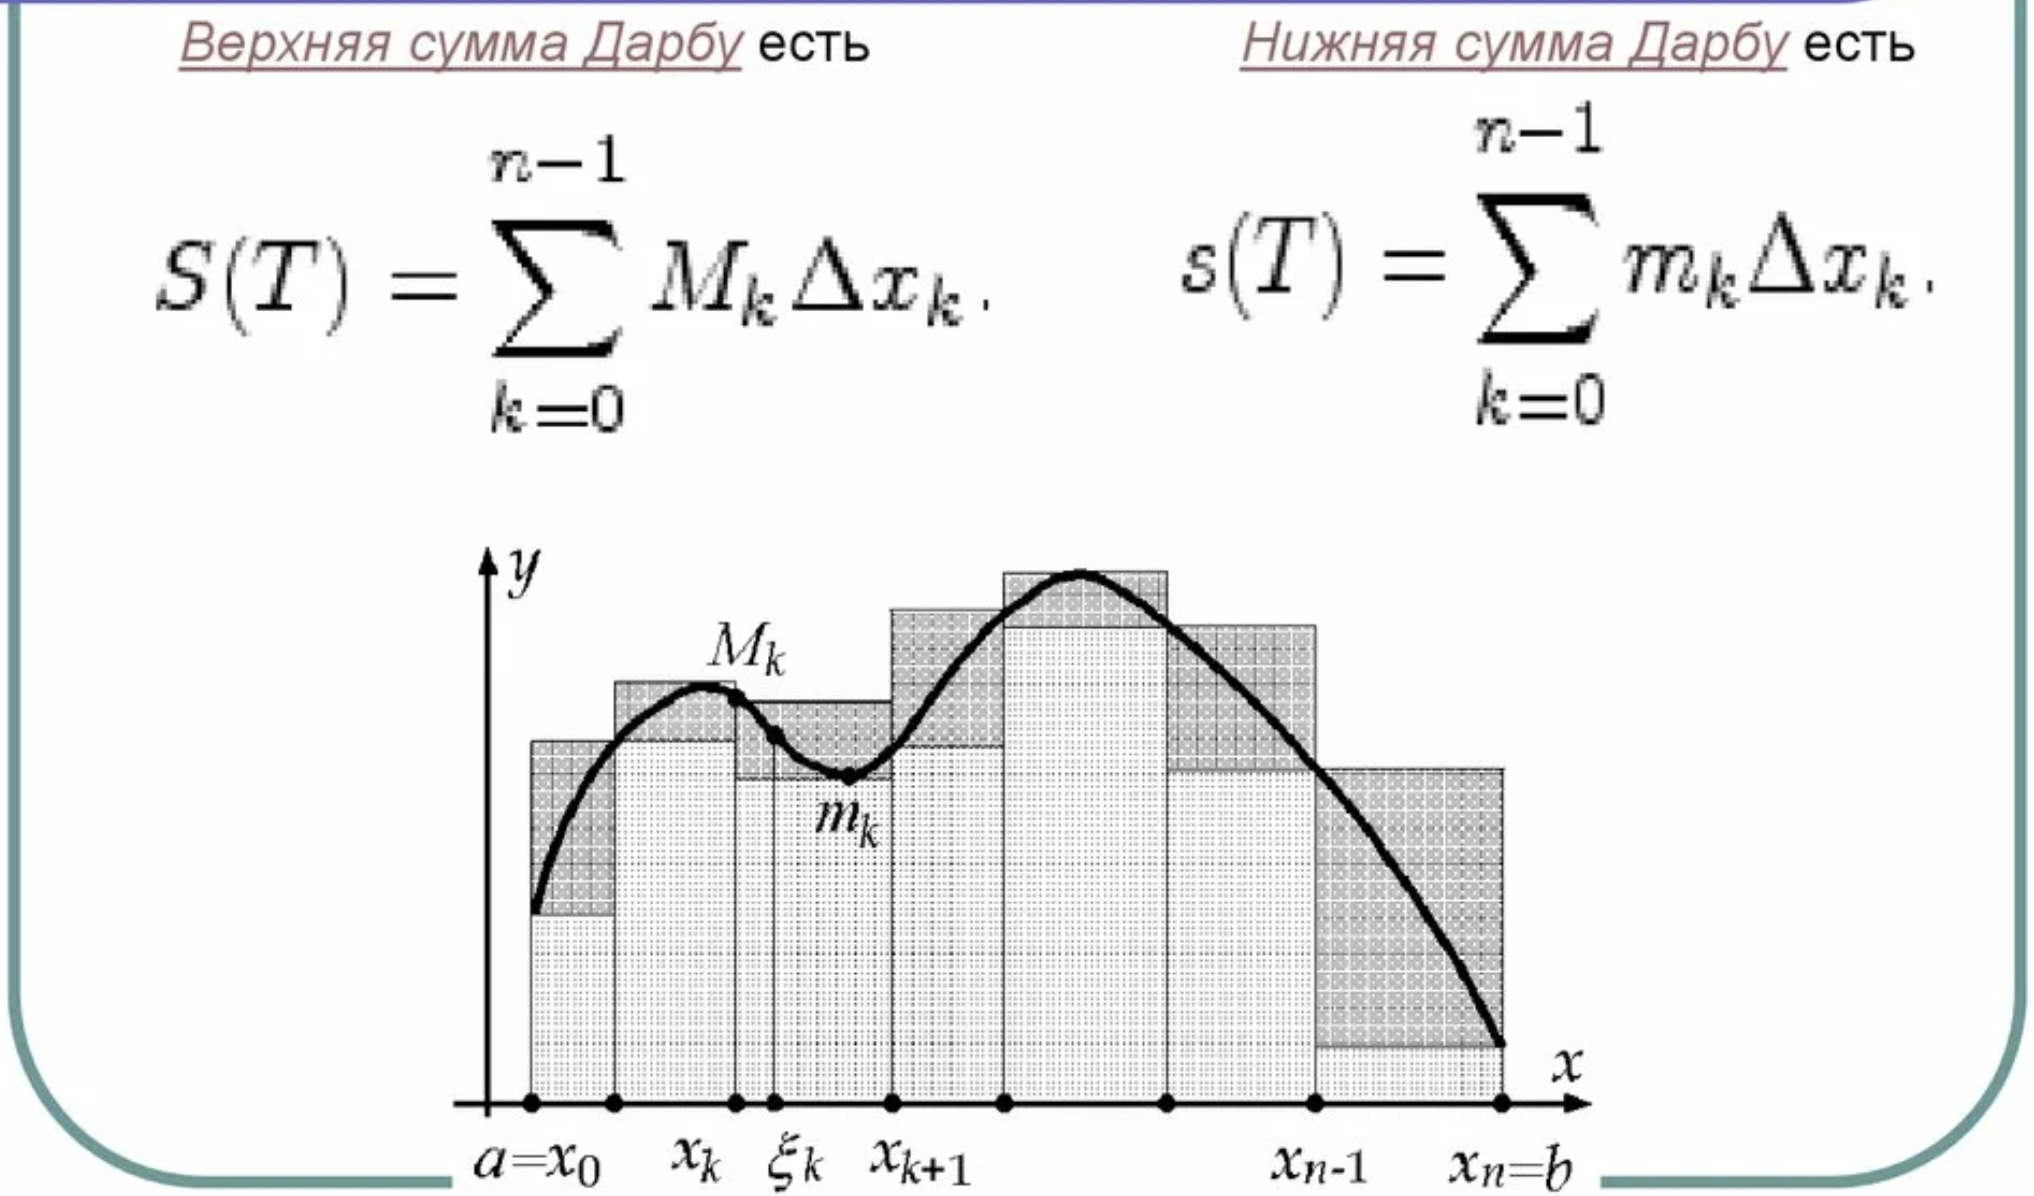
\includegraphics[width=0.42\textwidth]{darbu.png}
    \nopagebreak
    \\ \vspace{0.3em} \small\itshape Рис. 11.1: А вот и они
\end{center}

\begin{itemize}
    \item \textbf{Монотонность:} Добавление точки делит один столбик на два узких. Локальные минимумы на половинках могут стать только выше общего старого минимума. «Пол» приподнимается (площадь растет). Локальные максимумы — только ниже, «потолок» проседает (площадь падает).
    \item \textbf{Смысл оценки $p(M-m)\lambda(T)$:} При добавлении одной точки изменение площади происходит только внутри одного исходного отрезка. Его ширина не превышает $\lambda(T)$, а максимальный перепад высоты функции от самого дна до пика равен $(M-m)$. Значит, от одной точки мы выигрываем/теряем максимум площадь одного такого прямоугольника: $(M-m)\lambda(T)$. Если точек $p$ штук, то суммарный эффект не превысит $p(M-m)\lambda(T)$.
\end{itemize}

\paragraph{Доказательство в 4 коротких шага.}

\begin{enumerate}
    \item \textbf{Выделение изменяемого участка ($p=1$):}
    Пусть в разбиение $T$ добавлена одна точка $x^*$, попавшая внутрь отрезка $[x_{k-1}, x_k]$. Обозначим инфимумы на двух новых половинках как $m'_1$ и $m'_2$. Поскольку точная нижняя грань на подмножестве не может быть меньше грани на всем множестве, имеем: $m'_1 \ge m_k$ и $m'_2 \ge m_k$.
    
    Разность новых и старых нижних сумм возникает исключительно на этом отрезке:
    $$ s(f, T') - s(f, T) = m'_1 (x^* - x_{k-1}) + m'_2 (x_k - x^*) - m_k \Delta x_k $$

    \item \textbf{Алгебраический трюк с точкой $x^*$:}
    Распишем длину старого отрезка через тождественное добавление и вычитание точки $x^*$: $\Delta x_k = x_k - x_{k-1} = (x^* - x_{k-1}) + (x_k - x^*)$. Подставим это в формулу разности и сгруппируем члены при одинаковых скобках длины:
    $$ s(f, T') - s(f, T) = \underbrace{(m'_1 - m_k)}_{\ge 0} \underbrace{(x^* - x_{k-1})}_{> 0} + \underbrace{(m'_2 - m_k)}_{\ge 0} \underbrace{(x_k - x^*)}_{> 0} \ge 0 \implies s(f, T) \le s(f, T') $$
    Для верхних сумм аналогично через супремумы ($M'_1 \le M_k, M'_2 \le M_k$):
    $$ S(f, T) - S(f, T') = \underbrace{(M_k - M'_1)}_{\ge 0} (x^* - x_{k-1}) + \underbrace{(M_k - M'_2)}_{\ge 0} (x_k - x^*) \ge 0 \implies S(f, T') \le S(f, T) $$

    \item \textbf{Вывод оценки для одной точки:}
    Оценим сверху разность нижних сумм из предыдущего шага. Так как $m'_1 \le M$ (глобальный супремум), а $m_k \ge m$ (глобальный инфимум), то каждая разность инфимумов не превышает полный размах функции: $(m'_1 - m_k) \le M - m$ и $(m'_2 - m_k) \le M - m$. Вынесем $(M-m)$ за скобки:
    $$ s(f, T') - s(f, T) \le (M - m) \big[ (x^* - x_{k-1}) + (x_k - x^*) \big] = (M - m)\Delta x_k $$
    Учитывая, что длина любого отрезка не больше мелкости разбиения ($\Delta x_k \le \lambda(T)$), получаем:
    $$ s(f, T') - s(f, T) \le (M - m)\lambda(T) $$

    \item \textbf{Переход к произвольному числу $p$ точек:}
    Если добавляется $p$ точек, будем вводить их поочередно, выстраивая цепочку разбиений: $T = T_0 \subset T_1 \subset \dots \subset T_p = T'$. При каждом добавлении одной точки мелкость текущего разбиения не превосходит исходную: $\lambda(T_i) \le \lambda(T)$.
    Складывая $p$ полученных на каждом шаге одинаковых оценок, по правилу телескопической суммы имеем:
    $$ s(f, T') - s(f, T) = \sum_{i=1}^p \big(s(f, T_i) - s(f, T_{i-1})\big) \le \sum_{i=1}^p (M - m)\lambda(T) = p(M - m)\lambda(T) $$
    Доказательство для верхних сумм проводится зеркально. Лемма полностью доказана.
\end{enumerate}


% --- Вопрос 12 ---
\examquestion{12}{Критерий интегрируемости в терминах сумм Дарбу}
{Сформулируйте и проведите доказательство теоремы: Критерий интегрируемости Дарбу. Проработайте доказательство в обе стороны (необходимость и достаточность).}

\paragraph{Базовые понятия и обозначения.}
Для любого разбиения $T$ отрезка $[a, b]$ определены нижняя $s(f, T)$ и верхняя $S(f, T)$ суммы Дарбу.
\begin{itemize}
    \item \textbf{Интегралы Дарбу:} Нижним интегралом Дарбу $I_*$ называется супремум всех нижних сумм, а верхним интегралом $I^*$ — инфимум всех верхних сумм по всем возможным разбиениям:
    $$ I_* = \sup_{T} s(f, T), \quad I^* = \inf_{T} S(f, T) $$
    \item \textbf{Интегрируемость по Риману:} Ограниченная функция $f(x)$ называется интегрируемой по Риману ($f \in \mathcal{R}[a,b]$), если её верхний и нижний интегралы Дарбу совпадают. Их общее значение равно интегралу Римана: $I_* = I^* = I$.
    \item \textbf{Смысл оценки:} Разность $S(f, T) - s(f, T)$ — это суммарная площадь «зазоров» между накрывающей и вписанной ступенчатыми фигурами. Функция интегрируема тогда и только тогда, когда этот зазор можно сжать до сколь угодно малой величины $\varepsilon$.
\end{itemize}

\paragraph{Формулировка теоремы (Критерий Дарбу).}
Ограниченная на отрезке $[a, b]$ функция $f(x)$ интегрируема по Риману на этом отрезке тогда и только тогда, когда для любого $\varepsilon > 0$ существует такое разбиение $T$, при котором:
\begin{tcolorbox}[colback=white, colframe=black, boxrule=0.5pt, arc=0pt, borderline={0.5pt}{0pt}{black, dashed}]
$$ f \in \mathcal{R}[a,b] \iff \forall \varepsilon > 0 \;\; \exists T : \;\; S(f, T) - s(f, T) < \varepsilon $$
\end{tcolorbox}

\paragraph{Доказательство необходимости ($\implies$).}
Пусть функция интегрируема, то есть $I_* = I^* = I$. Зафиксируем произвольное $\varepsilon > 0$.
\begin{enumerate}
    \item По определению супремума, для величины $\frac{\varepsilon}{2}$ найдется разбиение $T_1$, нижняя сумма которого близка к $I$:
    $$ s(f, T_1) > I - \frac{\varepsilon}{2} $$
    \item По определению инфимума, для величины $\frac{\varepsilon}{2}$ найдется разбиение $T_2$, верхняя сумма которого близка к $I$:
    $$ S(f, T_2) < I + \frac{\varepsilon}{2} $$
    \item Построим общее измельчение $T = T_1 \cup T_2$. По лемме об изменении сумм, при добавлении новых точек нижняя сумма может только вырасти, а верхняя — только уменьшиться. Тогда справедливы два раздельных неравенства:
    $$ s(f, T) \ge s(f, T_1) > I - \frac{\varepsilon}{2} \implies -s(f, T) < -I + \frac{\varepsilon}{2} $$
    $$ S(f, T) \le S(f, T_2) < I + \frac{\varepsilon}{2} $$
    Сложим эти два неравенства для одного и того же разбиения $T$:
    $$ S(f, T) - s(f, T) < \left(I + \frac{\varepsilon}{2}\right) + \left(-I + \frac{\varepsilon}{2}\right) = \varepsilon $$
\end{enumerate}
Необходимость доказана.

\paragraph{Доказательство достаточности ($\impliedby$).}
Пусть условие выполнено: для любого $\varepsilon > 0$ существует разбиение $T$, при котором $S(f, T) - s(f, T) < \varepsilon$.

По определению интегралов Дарбу как точных граней, для абсолютно любого разбиения $T$ выполнены стандартные ограничения: $s(f, T) \le I_*$ и $I^* \le S(f, T)$. Избавимся от тройного неравенства и запишем это в виде двух простых утверждений:
\begin{enumerate}
    \item Так как $I^* \le S(f, T)$ и $-I_* \le -s(f, T)$, мы можем оценить разность интегралов сверху через разность сумм на данном разбиении:
    $$ I^* - I_* \le S(f, T) - s(f, T) $$
    \item Поскольку по условию эта разность сумм меньше $\varepsilon$, получаем:
    $$ 0 \le I^* - I_* < \varepsilon $$
\end{enumerate}
Постоянная величина $I^* - I_*$ неотрицательна и при этом строго меньше любого сколь угодно малого положительного числа $\varepsilon$. Это возможно только если эта разность равна нулю:
$$ I^* - I_* = 0 \implies I_* = I^* $$
По определению это означает, что функция интегрируема по Риману. Достаточность доказана.

% --- Вопрос 13 ---
\examquestion{13}{Интегрируемость непрерывных функций}
{Сформулируйте и докажите теорему об интегрируемости по Риману любой функции, непрерывной на сегменте $[a, b]$ ($C[a,b]\subset\mathcal{R}[a,b]$). Покажите, на каком именно этапе доказательства и для чего необходимо применять теорему Кантора о равномерной непрерывности.}

\paragraph{Используемые теоремы.}
Для доказательства опираемся на три факта:
\begin{itemize}
    \item \textbf{Вторая теорема Вейерштрасса:} Непрерывная на отрезке функция всегда достигает на нем своих точных граней (максимума и минимума).
    \item \textbf{Теорема Кантора:} Непрерывная на замкнутом отрезке функция равномерно непрерывна. То есть для любого $\varepsilon > 0$ существует единое $\delta > 0$, такое что при $|x' - x''| < \delta$ всегда выполняется $|f(x') - f(x'')| < \varepsilon$.
    \item \textbf{Критерий Дарбу:} Функция интегрируема, если $\forall \varepsilon > 0 \exists T: S(f, T) - s(f, T) < \varepsilon$.
\end{itemize}

\paragraph{Формулировка теоремы.}
Если функция $f(x)$ непрерывна на сегменте $[a, b]$, то она интегрируема по Риману на этом сегменте.

\paragraph{Тезисное доказательство.}
\begin{enumerate}
    \item Зададим произвольное $\varepsilon > 0$. 
    \item \textbf{Применяем теорему Кантора:} Для величины $\frac{\varepsilon}{b-a} > 0$ существует \textit{общее} $\delta > 0$, такое что для любых точек, расстояние между которыми меньше $\delta$, разность значений функции строго меньше $\frac{\varepsilon}{b-a}$.
    \item Возьмем любое разбиение $T$ с мелкостью $\lambda(T) < \delta$. Это значит, что длина каждого $k$-го отрезка $\Delta x_k < \delta$.
    \item На каждом отрезке $[x_{k-1}, x_k]$ функция непрерывна. По \textbf{теореме Вейерштрасса} она достигает внутри него инфимума $m_k$ и супремума $M_k$ в конкретных точках $x'_k$ и $x''_k$.
    \item Так как обе эти точки лежат внутри одного отрезка, расстояние между ними меньше $\delta$. Значит, размах функции на этом участке ограничен:
    $$ M_k - m_k < \frac{\varepsilon}{b-a} $$
    \item Составим разность сумм Дарбу для всего разбиения и заменим скобки с размахом на нашу оценку:
    $$ S(f, T) - s(f, T) = \sum_{k=1}^n (M_k - m_k)\Delta x_k < \sum_{k=1}^n \frac{\varepsilon}{b-a}\Delta x_k $$
    \item Выносим константу за сумму. Сумма длин всех подотрезков равна $(b-a)$:
    $$ \frac{\varepsilon}{b-a} \sum_{k=1}^n \Delta x_k = \frac{\varepsilon}{b-a}(b-a) = \varepsilon $$
    \item Получили $S(f, T) - s(f, T) < \varepsilon$. По критерию Дарбу функция интегрируема.
\end{enumerate}

\paragraph{Интуитивный смысл («на пальцах»).}
Обычная непрерывность гарантирует, что график плавный, но масштаб этой плавности (своё $\delta$) в каждой точке может быть разным. Теорема Кантора спасает ситуацию: она разрешает выбрать \textbf{одно общее, самое строгое $\delta$} для всего отрезка. Если нарезать ось $x$ на кусочки мельче этого $\delta$, колебания графика внутри \textit{каждой} ячейки одновременно станут микроскопическими. Суммарная площадь "зазоров" между ступенчатыми фигурами Дарбу схлопнется до нуля, и интеграл возьмется.



% --- Вопрос 14 ---
\examquestion{14}{Интегрируемость монотонных функций}
{Сформулируйте и докажите теорему об интегрируемости монотонной функции на сегменте $[a, b]$. Проведите доказательство через телескопическую оценку разности сумм Дарбу. Проведите сравнительный анализ: почему для монотонных функций не нужна теорема Кантора?}

\paragraph{Формулировка теоремы.}
Если функция $f(x)$ монотонна на сегменте $[a, b]$, то она интегрируема на этом сегменте.

\paragraph{Доказательство.}
Пусть $f(x)$ монотонно не убывает. Если $f(a) = f(b)$, функция константна и интегрируема. Рассмотрим случай $f(b) > f(a)$.

Зададим $\varepsilon > 0$. Разделим $[a, b]$ на $n$ равных частей длиной $\Delta x = \frac{b-a}{n}$. 
Из-за монотонности точные грани на каждом отрезке $[x_{k-1}, x_k]$ достигаются на его концах:
$$ m_k = f(x_{k-1}), \quad M_k = f(x_k) $$

Разность сумм Дарбу принимает вид:
$$ S(f, T) - s(f, T) = \sum_{k=1}^n (M_k - m_k) \Delta x = \frac{b-a}{n} \sum_{k=1}^n (f(x_k) - f(x_{k-1})) $$

Сумма внутри — телескопическая: все промежуточные значения $f(x_k)$ сокращаются, остаются только края:
$$ \sum_{k=1}^n (f(x_k) - f(x_{k-1})) = f(x_n) - f(x_0) = f(b) - f(a) $$

Итоговая разность:
$$ S(f, T) - s(f, T) = \frac{b-a}{n} (f(b) - f(a)) $$

Для любого заданного $\varepsilon$ мы можем выбрать столь большое количество разбиений $n$, чтобы это выражение стало меньше $\varepsilon$. Так как при любом $n$ мы можем подобрать такое разбиение, условие критерия Дарбу выполняется. Интегрируемость доказана.

\paragraph{Почему не нужна теорема Кантора?}
Для непрерывных функций мы не знаем, где внутри отрезка лежат экстремумы, поэтому вынуждены принудительно ограничивать колебания через равномерную непрерывность (теорему Кантора). 
У монотонной функции экстремумы всегда «сидят» на концах отрезков. Из-за этого суммарная ошибка разбиения зависит только от разности значений в крайних точках всего сегмента $[a, b]$, а не от «поведения» функции внутри. Монотонность сама по себе жестко ограничивает накопленную погрешность: сколько бы разрывов ни было внутри, они все «схлопываются» при телескопическом сокращении.

% --- Вопрос 15 ---
\examquestion{15}{Интегрируемость функций с конечным числом разрывов}
{Сформулируйте и докажите теорему об интегрируемости ограниченной функции, имеющей конечное число точек разрыва на сегменте $[a, b]$. Примените метод «изоляции». Обоснуйте важность ограниченности функции (пример $1/x$).}

\paragraph{Формулировка теоремы.}
Если функция $f(x)$ ограничена на сегменте $[a, b]$ и имеет на нем конечное число точек разрыва, то она интегрируема на этом сегменте.

\paragraph{Доказательство (Метод «изоляции»).}
Пусть функция ограничена: существует такое число $M>0$, что $-M \le f(x) \le M$ для всех $x \in [a,b]$ (функция зажата в коридоре высотой $2M$). 

Проведем доказательство для одной точки разрыва $c \in (a, b)$ (для $k$ точек алгоритм аналогичен). Зададим произвольное $\varepsilon > 0$.

\begin{enumerate}
    \item \textbf{Шаг 1. Изолируем разрыв.} Окружим точку $c$ интервалом $(c - \delta, c + \delta)$. Длина этого центрального отрезка разбиения равна $\Delta x_c = (c + \delta) - (c - \delta) = 2\delta$.
    \item \textbf{Шаг 2. Выбираем ширину.} Мы сами вправе выбрать $\delta$ сколь угодно малым. Сожмем его так, чтобы выполнялось условие: $4M\delta < \frac{\varepsilon}{2}$.
    \item \textbf{Шаг 3. Работаем с остатком.} Вне этого интервала остаются два чистых сегмента: $[a, c - \delta]$ и $[c + \delta, b]$. На них функция непрерывна, а значит, интегрируема. По критерию Дарбу для них найдутся такие разбиения $T_1$ и $T_2$, что разности их сумм ничтожно малы:
    $$ S(T_1) - s(T_1) < \frac{\varepsilon}{4} \quad \text{и} \quad S(T_2) - s(T_2) < \frac{\varepsilon}{4} $$
\end{enumerate}

Объединим разбиения $T_1, T_2$ и центральный отрезок $[c - \delta, c + \delta]$ в единое полное разбиение $T$ всего сегмента $[a, b]$. Полная разность сумм Дарбу распадается на три части:
$$ S(f, T) - s(f, T) = \underbrace{\big(S(T_1) - s(T_1)\big)}_{< \varepsilon/4} + \underbrace{(M_c - m_c)\Delta x_c}_{\text{окрестность } c} + \underbrace{\big(S(T_2) - s(T_2)\big)}_{< \varepsilon/4} $$

\paragraph{Подробная оценка центрального слагаемого:}
\begin{itemize}
    \item Так как функция зажата в пределах от $-M$ до $+M$, её максимальное значение $M_c \le M$, а минимальное $m_c \ge -M$. 
    \item Значит, максимальный размах (колебание) функции на отрезке не может превысить: $(M_c - m_c) \le M - (-M) = 2M$.
    \item Длина отрезка равна $\Delta x_c = 2\delta$.
    \item Перемножаем их: $(M_c - m_c)\Delta x_c \le 2M \cdot 2\delta = 4M\delta$.
    \item А так как на Шаге 2 мы сами зафиксировали, что $4M\delta < \frac{\varepsilon}{2}$, то центральное слагаемое железно меньше $\frac{\varepsilon}{2}$.
\end{itemize}

Собираем все три части суммы вместе:
$$ S(f, T) - s(f, T) < \frac{\varepsilon}{4} + \frac{\varepsilon}{2} + \frac{\varepsilon}{4} = \varepsilon $$
Разность сумм Дарбу оказалась меньше $\varepsilon$. По критерию Дарбу функция интегрируема.

\vspace{0.5em}
\begin{center}
\begin{tikzpicture}[scale=0.9, every node/.style={scale=0.9}]
    \draw[->, thick] (0,0) -- (6,0) node[right] {$x$};
    \draw[->, thick] (0,0) -- (0,3) node[above] {$y$};
    
    % График функции с разрывом
    \draw[thick, blue] (0.5, 2) .. controls (1.5, 2) .. (2.5, 1);
    \draw[thick, blue] (3.5, 2.5) .. controls (4.5, 2.5) .. (5.5, 1.5);
    \filldraw[blue] (2.5, 1) circle (2pt);
    \draw[blue, fill=white, thick] (3.5, 2.5) circle (2pt);
    
    % Изолирующий пакет
    \draw[dashed, red, fill=red!10, thick] (2.5,0) rectangle (3.5, 2.6);
    \node[red, align=center] at (3, 3) {Изолирующий \\ пакет $\Delta x_c$};
    
    % Подписи
    \draw[thick] (2.5, 0.1) -- (2.5, -0.1) node[below] {$c-\delta$};
    \draw[thick] (3.5, 0.1) -- (3.5, -0.1) node[below] {$c+\delta$};
    \node[below=10pt, red] at (3, 0) {$c$};
\end{tikzpicture}
\end{center}
\vspace{0.5em}

\paragraph{Важность условия ограниченности (Пример $1/x$).}
Метод изоляции работает **только** если высота изолирующего прямоугольника ограничена константой $M$. Если функция улетает в бесконечность, метод ломается.
Рассмотрим функцию $f(x) = \frac{1}{x}$ на интервале $(0, 1)$, доопределив её в нулю ($f(0) = 0$). У неё одна точка разрыва ($x = 0$).

Для любого разбиения $T$ самый первый отрезок $[0, x_1]$ содержит разрыв. Точная верхняя грань функции на нём бесконечна: $M_1 = \sup_{[0, x_1]} \frac{1}{x} = +\infty$.
Из-за этого верхняя сумма Дарбу всегда «взрывается»:
$$ S(f, T) = \underbrace{M_1 \cdot \Delta x_1}_{+\infty} + \sum_{k=2}^n M_k \Delta x_k = +\infty $$
Разность $S(f,T) - s(f,T) = +\infty$. Критерий Дарбу не выполняется, интеграл Римана не существует.

\vspace{0.5em}
\begin{center}
\begin{tikzpicture}[scale=0.9, every node/.style={scale=0.9}]
    \draw[->, thick] (0,0) -- (5,0) node[right] {$x$};
    \draw[->, thick] (0,0) -- (0,4) node[above] {$y$};
    
    % График 1/x
    \draw[domain=0.25:4.5, smooth, variable=\x, thick, blue] plot ({\x}, {1/\x});
    
    % Бесконечный прямоугольник
    \draw[fill=red!20, thick] (0, 0) rectangle (1.2, 3.8);
    \draw[->, thick, red] (0.6, 2.5) -- (0.6, 4.2) node[above] {$M_1 \to +\infty$};
    \node[red, align=center] at (2.5, 3.0) {Площадь первого \\ пакета $\to \infty$};
    
    % Подписи
    \draw[thick] (1.2, 0.1) -- (1.2, -0.1) node[below] {$x_1$};
\end{tikzpicture}
\end{center}
\vspace{0.5em}